% Created 2015-09-30 Wed 22:00
\documentclass{article}
\usepackage[top=1in, bottom=1.in, left=1in, right=1in]{geometry}
  \usepackage[makeroom]{cancel}
\usepackage{verbatim}


\usepackage[utf8]{inputenc}
\usepackage{lmodern}
\usepackage[T1]{fontenc}
\usepackage{fixltx2e}
\usepackage{graphicx}
\usepackage{longtable}
\usepackage{float}
\usepackage{wrapfig}
\usepackage{rotating}
\usepackage[normalem]{ulem}
\usepackage{amsmath}
\usepackage{textcomp}
\usepackage{marvosym}
\usepackage{wasysym}
\usepackage{amssymb}
\usepackage{amsmath}
\usepackage[version=3]{mhchem}
\usepackage[numbers,super,sort&compress]{natbib}
\usepackage{natmove}
\usepackage{url}
\usepackage{minted}
\usepackage{underscore}
\usepackage[linktocpage,pdfstartview=FitH,colorlinks,
linkcolor=blue,anchorcolor=blue,
citecolor=blue,filecolor=blue,menucolor=blue,urlcolor=blue]{hyperref}
\usepackage{attachfile}
\author{Abhishek Bagusetty}
\date{\today}
\title{24-623 2015 HM2}
\begin{document}

\maketitle

\section{Problem 1}
\label{sec-1}
\subsection{(a)}
\label{sec-1-1}
\subsubsection{(1)}
\label{sec-1-1-1}
\begin{equation}
\frac{1}{2m_{i}}\frac{\partial|\boldsymbol{p_{i}}|^2}{\partial\boldsymbol{p_{i}}} = \frac{\boldsymbol{p_{i}}}{m_{i}}
\label{eq:1.1a}}
\end{equation}

$$|\boldsymbol{p_{i}}| = \sqrt{p_{x}^2+p_{y}^2+p_{z}^2}$$

\begin{equation}
\implies \frac{1}{2m_{i}} \frac{\partial|\boldsymbol{p_{i}}|^2}{\partial\boldsymbol{|p_{i}}|}
\frac{\partial|\boldsymbol{p_{i}}|}{\partial\boldsymbol{p_{i}}}
\end{equation}

\begin{equation}
\implies \cancel{2}|\boldsymbol{p_{i}}| \frac{1}{\cancel{2}m_{i}} \frac{\partial|\boldsymbol{p_{i}}|}{\partial\boldsymbol{p_{i}}} = \frac{|\boldsymbol{p_{i}}|}{m_{i}} \frac{\partial|\boldsymbol{p_{i}}|}{\partial\boldsymbol{p_{i}}}
\end{equation}

\begin{equation}
\implies \cancel{2}|\boldsymbol{p_{i}}| \frac{1}{\cancel{2}m_{i}} \frac{\partial|\boldsymbol{p_{i}}|}{\partial\boldsymbol{p_{i}}} = \frac{|\boldsymbol{p_{i}}|}{m_{i}} \frac{\partial|\boldsymbol{p_{i}}|}{\partial\boldsymbol{p_{i}}}
\end{equation}

\begin{equation}
\implies \frac{|\boldsymbol{p_{i}}|}{m_{i}} \frac{\partial|\boldsymbol{p_{i}}|}{\partial\boldsymbol{p_{i}}} = \frac{|\boldsymbol{p_{i}}|}{m_{i}} \Big( \frac{\partial \sqrt{p_{i,x}^2 + p_{i,y}^2 + p_{i,z}^2}}{\partial p_{x}}\boldsymbol{\hat i} + \frac{\partial \sqrt{p_{i,x}^2 + p_{i,y}^2 + p_{i,z}^2}}{\partial p_{y}}\boldsymbol{\hat j} + \frac{\partial \sqrt{p_{i,x}^2 + p_{i,y}^2 + p_{i,z}^2}}{\partial p_{z}}\boldsymbol{\hat k} \Big)
\end{equation}

\begin{equation}
\implies \frac{|\boldsymbol{p_{i}}|}{m_{i}} \frac{1}{\sqrt{p_{i,x}^2 + p_{i,y}^2 + p_{i,z}^2}} \Big( p_{i,x} \boldsymbol{\hat i} + p_{i,y} \boldsymbol{\hat j} + p_{i,z} \boldsymbol{\hat k} \Big) = \frac{\cancel{|\boldsymbol{p_{i}}|}}{m_{i}} \frac{1}{\cancel{|\boldsymbol{p_{i}}|}} \boldsymbol{p_{i}}
\end{equation}

\begin{equation}
\boxed{ \frac{1}{2m_{i}}\frac{\partial|\boldsymbol{p_{i}}|^2}{\partial\boldsymbol{p_{i}}} = \frac{\boldsymbol{p_{i}}}{m_{i}} }
\end{equation}

\subsubsection{(2)}
\label{sec-1-1-2}
\begin{equation}
\frac{\partial r_{ij}}{\partial \boldsymbol{r_{ij}}} = \frac{\boldsymbol{r_{ij}}}{r_{ij}}
\end{equation}

$$ \boldsymbol{r_{ij}} = \boldsymbol{r_{i}} - \boldsymbol{r_{j}} = r_{ij,x}\boldsymbol{\hat i} + r_{ij,y}\boldsymbol{\hat j} + r_{ij,z}\boldsymbol{\hat k} $$

$$ r_{ij} = \sqrt{r_{ij,x}^2 + r_{ij,y}^2 + r_{ij,z}^2} $$

\begin{equation}
\implies \frac{\partial r_{ij}}{\partial \boldsymbol{r_{ij}}} = \frac{\partial r_{ij}}{\partial r_{ij}} \frac{\partial r_{ij}}{\partial \boldsymbol{r_{ij}}}
\end{equation}

\begin{equation}
\implies \frac{\partial r_{ij}}{\partial \boldsymbol{r_{ij}}} = \frac{\partial r_{ij}}{\partial \boldsymbol{r_{ij}}}
\end{equation}

\begin{equation}
\implies \frac{\partial r_{ij}}{\partial \boldsymbol{r_{ij}}} = \frac{\partial \sqrt{r_{ij,x}^2 + r_{ij,y}^2 + r_{ij,z}^2}}{\partial r_{ij,x}} \boldsymbol{\hat i} + \frac{\partial \sqrt{r_{ij,x}^2 + r_{ij,y}^2 + r_{ij,z}^2}}{\partial r_{ij,y}} \boldsymbol{\hat j} + \frac{\partial \sqrt{r_{ij,x}^2 + r_{ij,y}^2 + r_{ij,z}^2}}{\partial r_{ij,z}} \boldsymbol{\hat k}
\end{equation}

\begin{equation}
\implies \frac{\partial r_{ij}}{\partial \boldsymbol{r_{ij}}} = \frac{1}{\sqrt{r_{ij,x}^2 + r_{ij,y}^2 + r_{ij,z}^2}} (r_{ij,x} \boldsymbol{\hat i} + r_{ij,y} \boldsymbol{\hat j} + r_{ij,z} \boldsymbol{\hat k})
\end{equation}

\begin{equation}
\boxed{ \frac{\partial r_{ij}}{\partial \boldsymbol{r_{ij}}} = \frac{\boldsymbol{r_{ij}}}{r_{ij}} }
\end{equation}

\subsubsection{(3)}
\label{sec-1-1-3}

\subsection{(b)}
\label{sec-1-2}
Forces at $(t+\Delta t)$ are computed in the third step will be same as the force in the first step of the next time step, hence establishing a time line continuity. The evolution of parameter (positions and velocities) has to be \textbf{reversible}.

These are the equations marching forward in time :
$$ v_{i,x}(t+\Delta t/2) = v_{i,x}(t) + F_{i,x}(t)\Delta t/(2m_{i})$$
$$ r_{i,x}(t+\Delta t) = r_{i,x}(t) + v_{i,x}(t+\Delta t/2)\Delta t $$
$$ v_{i,x}(t+\Delta t) = v_{i,x}(t+\Delta t/2) + F_{i,x}(t+\Delta t)\Delta t/(2m_{i}) $$


These are the equations marching backward in time by replacing $\Delta t$ by $-\Delta t$:
$$ v_{i,x}(t-\Delta t/2) = v_{i,x}(t) - F_{i,x}(t)\Delta t/(2m_{i})$$
$$ r_{i,x}(t-\Delta t) = r_{i,x}(t) + v_{i,x}(t-\Delta t/2)\Delta t $$
$$ v_{i,x}(t-\Delta t) = v_{i,x}(t-\Delta t/2) + F_{i,x}(t-\Delta t)\Delta t/(2m_{i}) $$

where $(t-\Delta t)$ is t for the previous time step, hence establishing reversibility for the velocity verlet scheme.

\section{Problem 2}
\label{sec-2}
\subsection{(a)}
\label{sec-2-1}
\subsection{(b)}
\label{sec-2-2}
Starting with Hamiltonian equations of motion and solving for position and velocity,

\begin{equation}
\dot{p} = -\frac{dU_{s}}{dx}
\end{equation}

$$U_{s} = x^2/2 $$

$$ \dot{p} = -x$$

$$ \dot{v} = -x$$

\begin{equation}
\frac{dv}{dt} = \frac{d^2x}{dt^2} = -x
\end{equation}

The above equation is a second order linear differential equation,
Solution to x is given by,

\begin{equation}
\boxed{x(t) = C_{2}sin(t) + C_{1}cos(t)}
\end{equation}
where C$_{\text{1}}$ and C$_{\text{2}}$ are the integration constants.

After using the initial conditions for x(0) = 0 and v(0) = $\sqrt 2$, the constants are determined as $C_{1} = x_{o}$ and $C_{2} = v_{o}$.

\begin{equation}
\boxed{x(t) = v_{o}sin(t) + x_{o}cos(t)}
\end{equation}

Differentiating the above equation boils to velocity
\begin{equation}
\boxed{v(t) = v_{o}cos(t) - x_{o}sin(t)}
\end{equation}

Using the conditions provided $x_{o} = 0$ and $v_{o} = \sqrt2$, the following profiles are obtained.

Energy is conserved based on the follwing analysis : 

\begin{equation}
E_{initial} = U(x) + K
\implies x^2/2 + frac{1}{2}v^2
at t=0, x=0, v=\sqrt 2,
\imples E_{i} = 1
\end{equation}

$$ E_{final} = x(t)^2/2 + \frac{1}{2}v(t)^2 $$
$$ \implies \frac{v_{o}^2sin^2(t)}{2} + \frac{1}{2}v_{o}^2cos^2(t) $$
$$ E_{f} = sin^2(t) + cos^2(t)  = 1 $$

$$ \Delta E = E_{final}-E_{initial} = 0 $$
Hence energy is conserved.

Momentum is not conserved because there is an evolution of the velocity at temporal scale.
\begin{equation}
\Delta p = m(v_{f} -v_{i})
\implies v_{o}cos(t)-v_{o}cos(0)
\implies v_{o}(cos(t)-1) \neq 0
\end{equation}


\begin{figure}[H]
\begin{centering}
\scalebox{0.55}{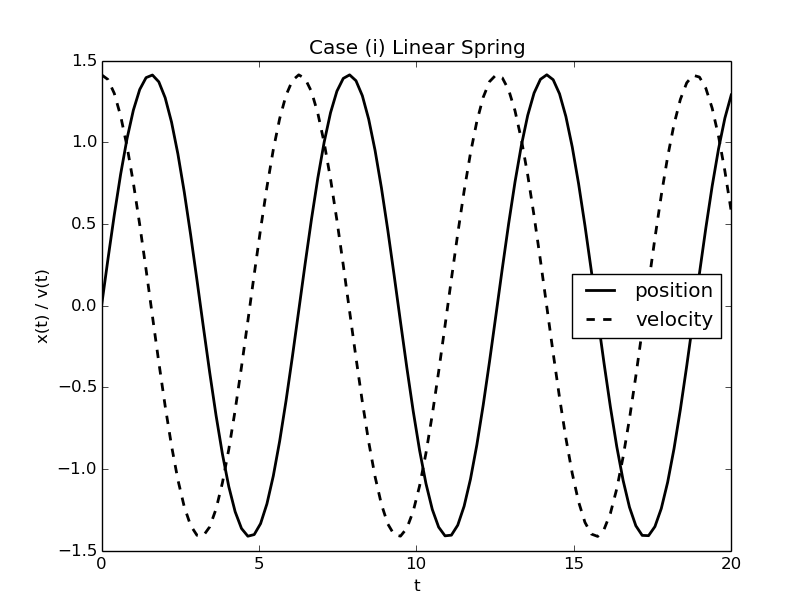
\includegraphics{./P2/figure1b.png}}
\caption{The figure shows the plot of energy for the MD simulation of LJ nano-particles over 1000 time frames.}
\label{fig:fig1}
\end{centering}
\end{figure}

\subsection{(c)}
\label{sec-2-3}
Time step is chosen based on the shape of the potential energy curve.The time period of the oscillations of the simple linear spring is T=2\PI. The time step is chosen to be 0.02T, so that about 50 time frames are evaluated to complete one oscillation. Hence a time step of 0.125 is chosen for the case (i) linear spring.

Position and velocity are computed using numerical integration of velocity-verlet scheme and the results are plotted against the analytical solutions from part (b) as shown below.
\begin{figure}[H]
\begin{centering}
\scalebox{0.55}{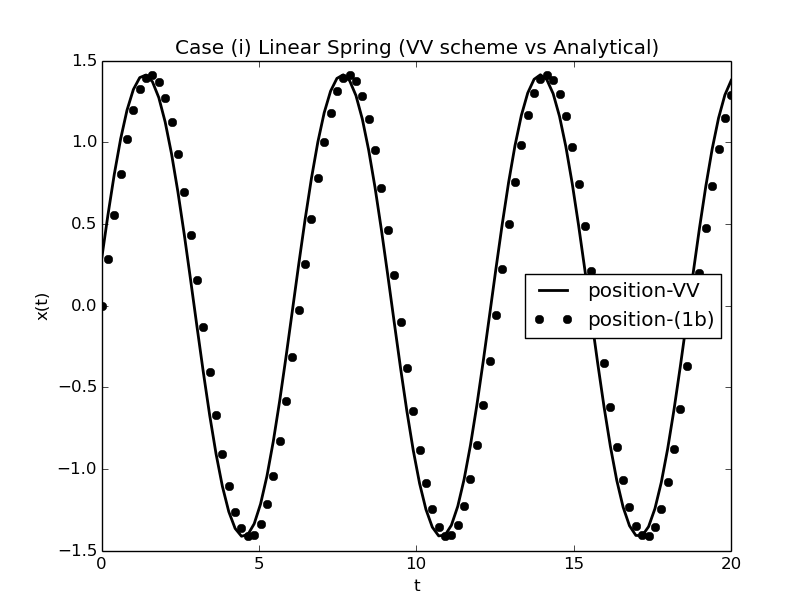
\includegraphics{./P2/figure1c1.png}}
\caption{The figure shows the plot of position calculated by numerical integration of velocity verlet scheme and also using the analytical expression from the above expression.}
\end{centering}
\end{figure}

\begin{figure}[H]
\begin{centering}
\scalebox{0.55}{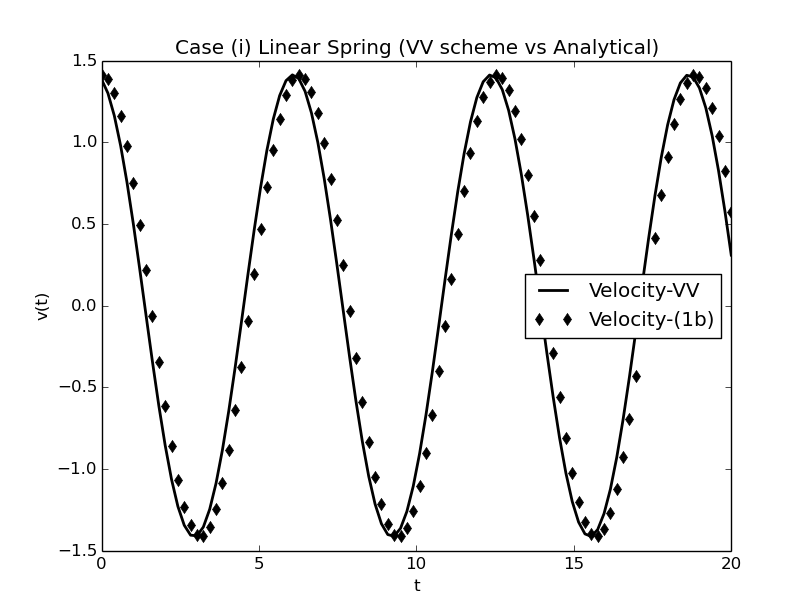
\includegraphics{./P2/figure1c2.png}}
\caption{The figure shows the plot of velocity calculated by numerical integration of velocity verlet scheme and also using the analytical expression from the above expression.}
\end{centering}
\end{figure}

\begin{figure}[H]
\begin{centering}
\scalebox{0.55}{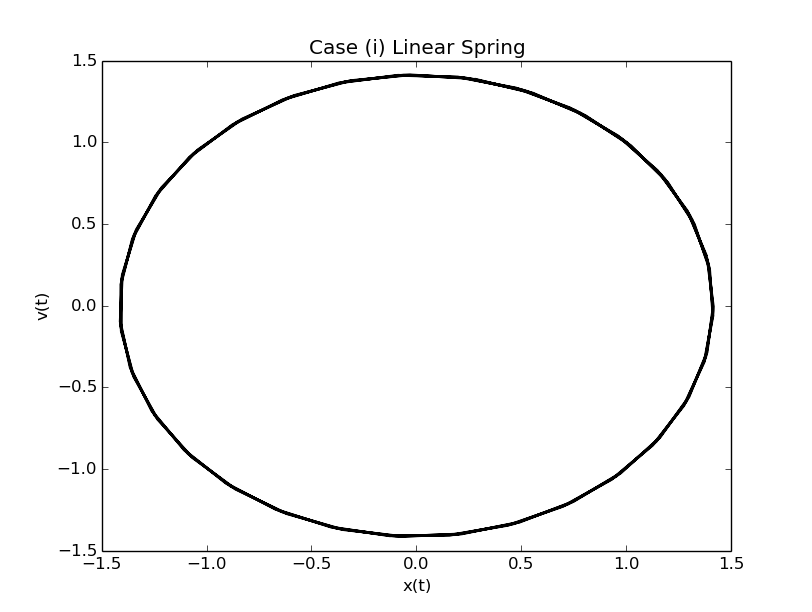
\includegraphics{./P2/figure1c3.png}}
\caption{The figure shows the plot of solution position and velocity on a constant energy manifold.}
\end{centering}
\end{figure}

\begin{figure}[H]
\begin{centering}
\scalebox{0.55}{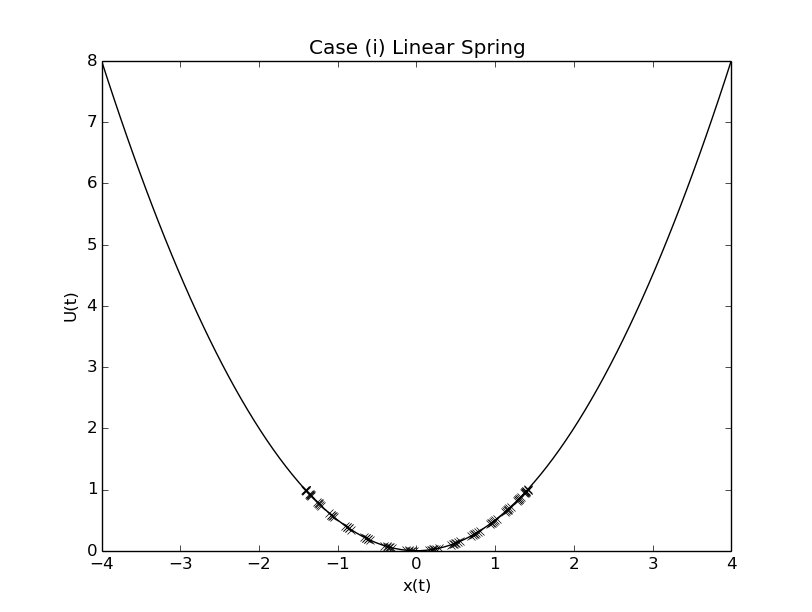
\includegraphics{./P2/figure1c4.png}}
\caption{The figure shows the plot of solution position points on the potential energy surface fucntion.}
\end{centering}
\end{figure}



\subsection{(c)}
\label{sec-2-4}
\subsection{(d)}
\label{sec-2-5}

\section{Problem 3}
\label{sec-3}
Velocities, positions and forces are the important variables allocated dynamically using double pointers. The size of the system or the number of atoms are determined dynamically.

Pair Energies, kinetic energy of the system is computed at every time unit to get better statistics. Center of mass(COM) is computed at each time frame to prove that there is no drift and also can also be visualized from the snapshots given below.

Components of momentum in x,y,z directions are computed and plotted as below. Data file is written which consists of potential, kinetic and total energy along with components of momentum at each time step for post processing.


\begin{figure}[H]
\begin{centering}
\scalebox{0.35}{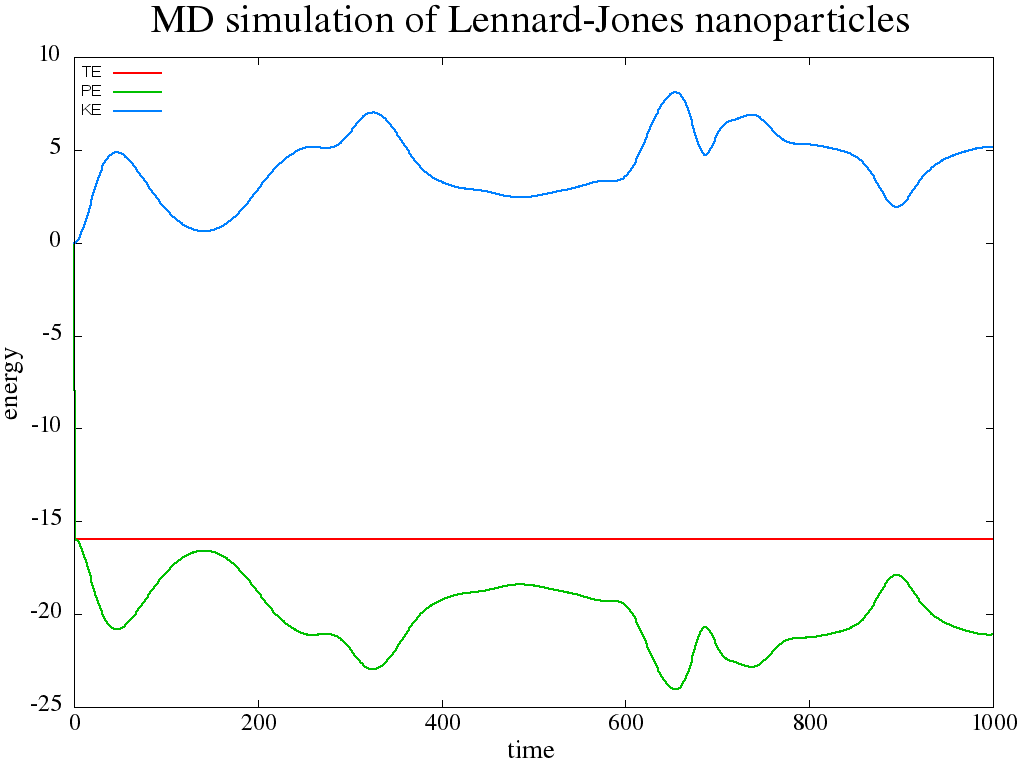
\includegraphics{./P3/LDmjsim.png}}
\caption{The figure shows the plot of energy for the MD simulation of LJ nano-particles over 1000 time frames.}
\label{fig:fig1}
\end{centering}
\end{figure}

\begin{figure}[H]
\begin{centering}
\scalebox{0.35}{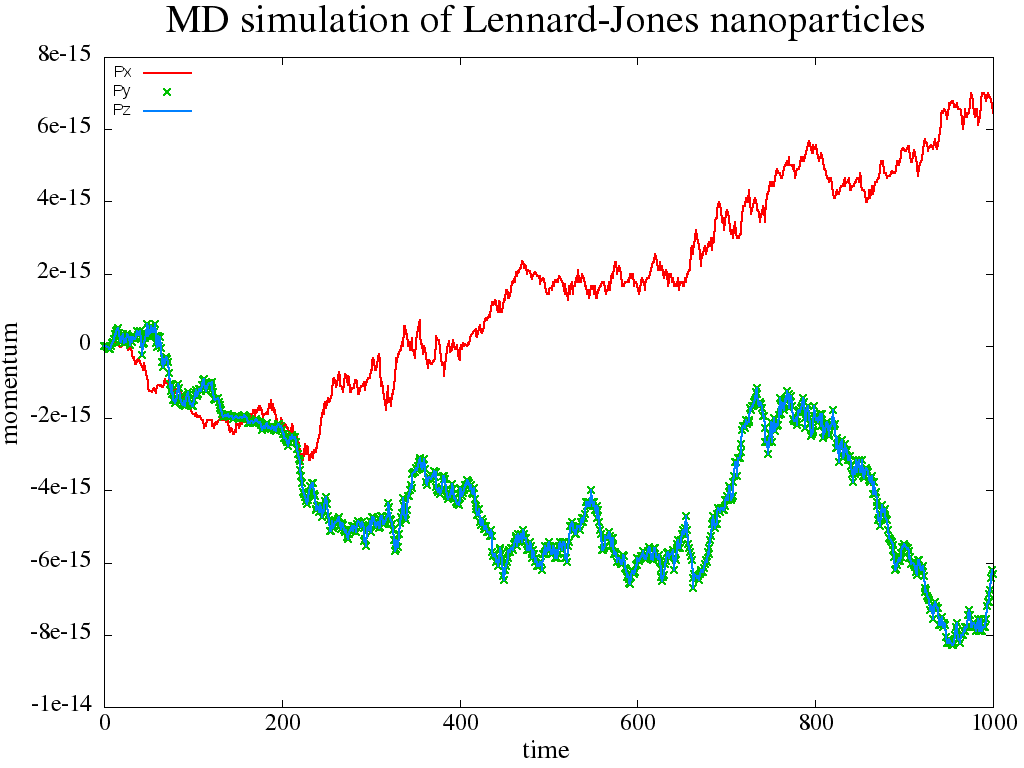
\includegraphics{./P3/LDmjsim1.png}}
\caption{The figure shows the plot of components of momentum for the MD simulation.}
\label{fig:fig1}
\end{centering}
\end{figure}


\begin{figure}[H]
\hfill
\subfigure{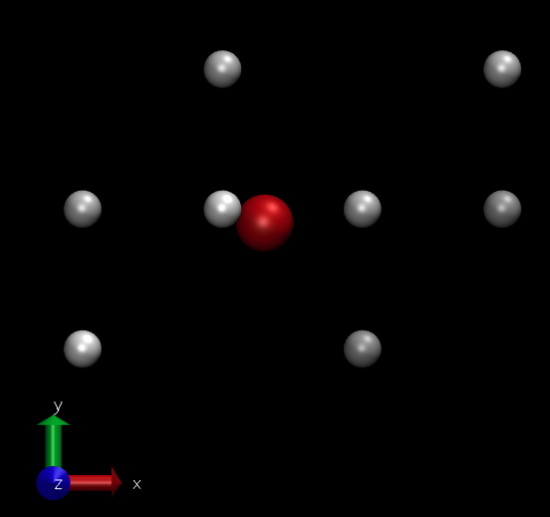
\includegraphics[widht=30mm,scale=0.20]{./t0.png}}
\hfill
\subfigure{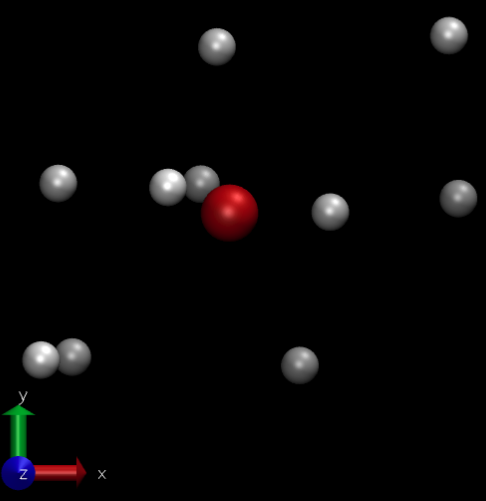
\includegraphics[widht=30mm,scale=0.20]{./t250.png}}
\hfill
\subfigure{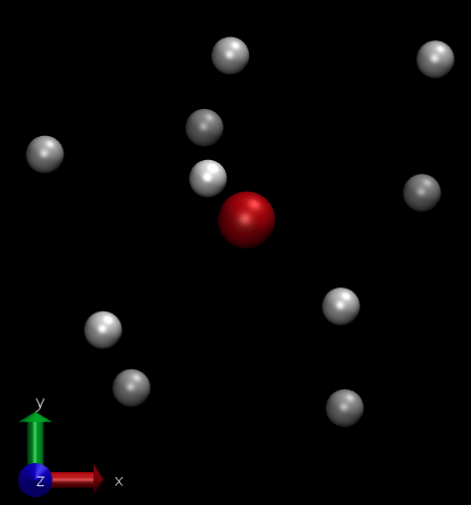
\includegraphics[widht=30mm,scale=0.20]{./t500.png}}
\hfill
\subfigure{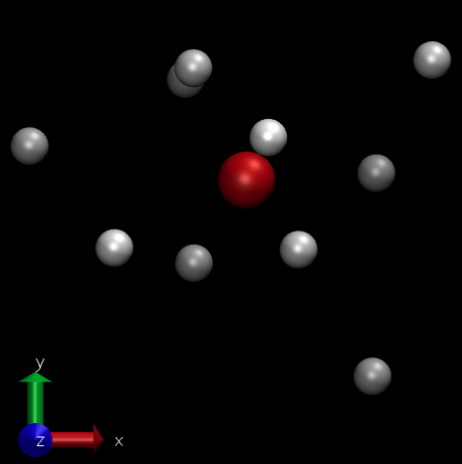
\includegraphics[widht=30mm,scale=0.22]{./t750.png}}
\hfill
\subfigure{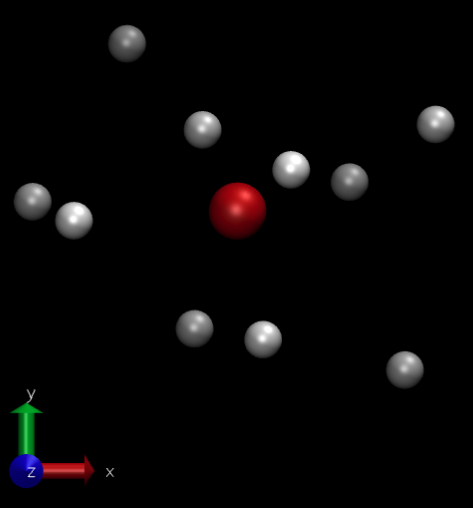
\includegraphics[widht=30mm,scale=0.20]{./t1000.png}}
\hfill
\caption{Snapshots of the configurations at various time units - 0,250,500,750,1000 (from left to right and bottom). Center of mass of the system is also shown in the configuration with red color.}
\end{figure}
% Emacs 24.4.1 (Org mode 8.2.10)
\end{document}